% =====================================================================
\chapter{Practical Experiments}
\label{ch:experiments}
% =====================================================================
Copy your own test images into \code{input/images/} and videos into \code{input/videos/}. Use your own recordings or images whose licence permits use. Do not use photographs of identifiable people without their consent. Each experiment lists the instruction, the tool the agent should choose, and what to verify. If the model chooses differently, that is a finding worth recording.

\begin{table}[ht]\centering\small
\begin{tabular}{@{}p{0.4cm}p{5.3cm}p{3.7cm}p{5.2cm}@{}}\toprule
\textbf{\#} & \textbf{Instruction} & \textbf{Expected tool} & \textbf{Verify}\\\midrule
1 & ``Give me the properties of \code{scene.png}.'' & \code{image_info} & Width, height, channels, size match \code{file}.\\
2 & ``Is \code{hallway.png} too dark? Fix it if needed.'' & \code{assess_image_quality}, then \code{enhance_low_light} & Reported mean intensity rises; parameters are reported.\\
3 & ``Remove salt-and-pepper noise from \code{noisy.png}.'' & \code{denoise_image} (median) & Isolated specks gone; edges intact. Ask the agent to compare median, Gaussian and bilateral if noise type is unknown.\\
4 & ``Read the text on \code{label.png} in English and Telugu.'' & \code{read_text} (\code{eng+tel}) & Compare against the true text; note the confidence.\\
5 & ``Extract one frame every 2 seconds from \code{walk.mp4}.'' & \code{extract_frames} & Count of saved frames $\approx$ duration$/2$.\\
6 & ``Detect objects in \code{street.png}.'' & \code{detect_objects} & Boxes drawn; zone and proximity sensible; sentence spoken.\\
7 & ``Analyse \code{walk.mp4} every 0.5 s.'' & \code{guide_video} & JSON timeline; mean latency reported.\\
8 & ``Run the full navigation pipeline on \code{corridor.png}.'' & \code{navigation_assist} & Steps list shows enhancement only if needed; WAV exists.\\
\bottomrule\end{tabular}
\caption{Agent experiments.}
\end{table}

\section{Controlled low-light experiment (measured)}
Real low-light footage has no clean reference, so image-quality metrics such as PSNR and SSIM cannot be computed. The standard remedy is a \emph{controlled} experiment: take a clean image, degrade it in a known way, enhance it, and compare with the original. The script \code{scripts/run_lowlight_experiment.py} does this with the astronaut photograph bundled with scikit-image, so it runs offline without extra downloads.
\begin{lstlisting}[style=sh]
python scripts/run_lowlight_experiment.py
\end{lstlisting}
The degradation is $I_{\text{dark}}=255\,(I/255)^{2.5}+\mathcal N(0,6^2)$ with a fixed random seed. Three enhancement settings are applied to the dark image.

\begin{figure}[ht]
\centering
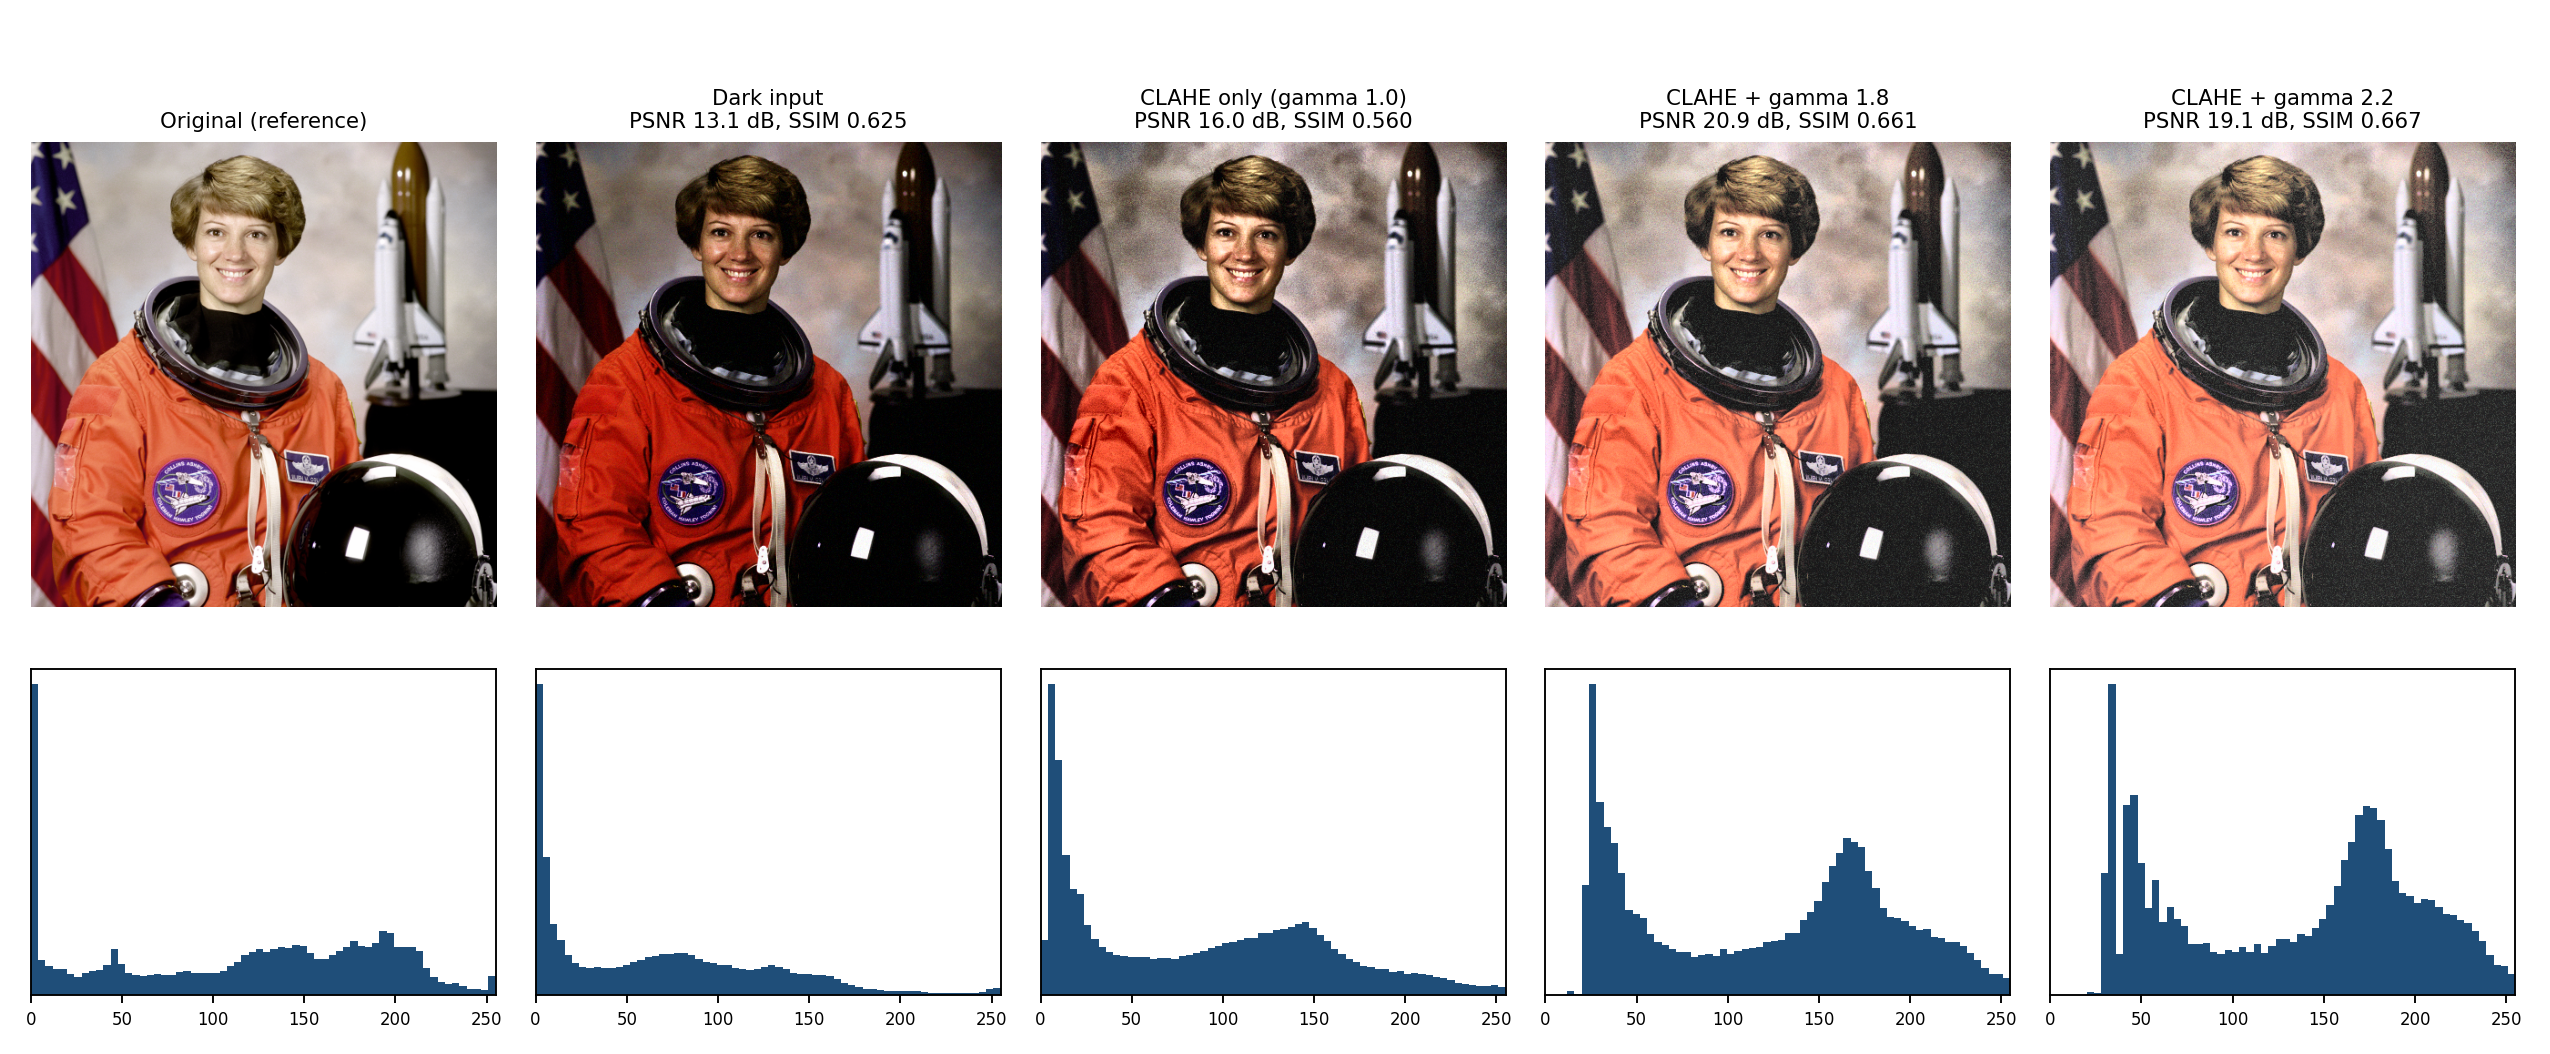
\includegraphics[width=\textwidth]{figures/lowlight_experiment.png}
\caption{Top: original, degraded input, and three enhancements. Bottom: grayscale histograms. PSNR and SSIM are computed against the original on the grayscale versions.}
\label{fig:lowlight}
\end{figure}

\begin{table}[ht]\centering\small
\begin{tabular}{@{}lrrr@{}}\toprule
\textbf{Image} & \textbf{PSNR (dB)} & \textbf{SSIM} & \textbf{Mean intensity}\\\midrule
Dark input & 13.05 & 0.625 & 65.7\\
CLAHE only ($\gamma=1.0$) & 16.04 & 0.560 & 86.7\\
CLAHE + gamma 1.8 & 20.88 & 0.661 & 121.7\\
CLAHE + gamma 2.2 & 19.11 & 0.668 & 133.6\\
\bottomrule\end{tabular}
\caption{Measured results (one image, one seed). Clip limit 2.0 and an $8\times8$ tile grid throughout.}
\end{table}

\paragraph{What the numbers do and do not say.}
\begin{itemize}
  \item CLAHE alone \emph{raised} PSNR but \emph{lowered} SSIM below the dark input. A likely explanation is that local contrast stretching also amplifies the added noise, which SSIM's structure term penalises; the evidence here (a single image) is suggestive, not conclusive. This is a good illustration of why one metric is never enough.
  \item Adding gamma 1.8 gave the highest PSNR; gamma 2.2 gave the highest SSIM but lower PSNR. There is no single ``best'' setting; it depends on the criterion, and the criterion should match the task (for example detection accuracy downstream).
  \item The result is for one synthetic degradation of one image. Do not generalise. Repeat over many images, several degradations and multiple seeds, and report mean and spread.
  \item PSNR and SSIM measure similarity to the original, not usefulness to a blind user or to a detector. The real test of an enhancement step is whether detection recall improves on genuinely dark frames (Chapter~\ref{ch:eval}).
\end{itemize}

% =====================================================================
\chapter{Evaluation}
\label{ch:eval}
% =====================================================================
\section{Image-quality metrics}
For a reference $I$ and a processed image $K$ of size $M\times N$:
\[
\text{MSE}=\frac{1}{MN}\sum_{x,y}\big[I(x,y)-K(x,y)\big]^2,\qquad
\text{PSNR}=10\log_{10}\frac{\text{MAX}_I^2}{\text{MSE}},
\]
with $\text{MAX}_I=255$ for 8-bit images (PSNR is infinite if the images are identical). SSIM compares luminance, contrast and structure in local windows:
\[
\text{SSIM}(x,y)=\frac{(2\mu_x\mu_y+C_1)(2\sigma_{xy}+C_2)}{(\mu_x^2+\mu_y^2+C_1)(\sigma_x^2+\sigma_y^2+C_2)}.
\]

\section{Detection metrics}
Match each prediction to a ground-truth box of the same class when their intersection over union exceeds a threshold (commonly $0.5$):
\[
\text{IoU}(A,B)=\frac{|A\cap B|}{|A\cup B|},\quad
P=\frac{TP}{TP+FP},\quad R=\frac{TP}{TP+FN},\quad F_1=\frac{2PR}{P+R}.
\]
For an assistive device \emph{recall on hazard classes} and \emph{false alarms per minute} usually matter more than overall accuracy. Report them separately for each lighting condition, because average performance hides failures in the dark.

\lstinputlisting[style=py,caption={\texttt{netra/metrics.py}},label=lst:metrics]{../netra/metrics.py}
\code{compare_images} takes the reference from \code{input/} and the processed image from \code{output/} (or \code{input/}); \code{simulate_low_light} creates the controlled degradation; \code{iou} and \code{precision_recall} are pure functions with unit tests. Greedy matching in descending confidence order is a simplification of the full mAP protocol; use the evaluation tools in your detection framework for published numbers.

\section{Task-level and system-level measures}
\begin{table}[ht]\centering\small
\begin{tabular}{@{}p{3.7cm}p{6cm}p{5cm}@{}}\toprule
\textbf{Measure} & \textbf{How to obtain it} & \textbf{Why it matters}\\\midrule
Hazard recall, precision & Annotate 200+ frames per condition; run \code{precision_recall} & Missed hazards and false alarms.\\
Zone accuracy & Compare predicted left/center/right with annotated side & Wrong side is worse than no message.\\
Proximity calibration & Place objects at measured distances; tabulate predicted class vs. true distance per class & Validates or replaces the area heuristic.\\
End-to-end latency & Time capture $\rightarrow$ detection $\rightarrow$ sentence $\rightarrow$ audio start & Stale guidance is misleading.\\
Throughput (FPS) & \code{benchmark_detector} on the target device & Feasibility on edge hardware.\\
False alarms per minute & Run on hazard-free footage & Alert fatigue.\\
Speech intelligibility & Listening tests with target users and languages & Usability.\\
Enhancement value & Detection recall with vs.\ without enhancement on real dark frames & The real test of Chapter~5 enhancement.\\
\bottomrule\end{tabular}
\caption{Evaluation plan for an assistive-vision prototype.}
\end{table}

\begin{table}[ht]\centering\small
\begin{tabular}{@{}lp{9cm}@{}}\toprule
\textbf{Stage} & \textbf{Latency budget (design target to verify, not a measurement)}\\\midrule
Capture and decode & as short as the camera allows\\
Quality check and enhancement & small compared with inference\\
Detection & dominant cost; depends on model, input size, device\\
Guidance sentence & negligible\\
Speech synthesis start & short for espeak-ng; longer for neural voices\\
\bottomrule\end{tabular}
\end{table}
Measure each stage separately on the target device, set an end-to-end target with your mobility instructors (how stale can a message be before it misleads?), and report percentiles, not only the mean.

\section{Testing and reproducibility}
The test suite checks path rejection, invalid arguments, quality flags, an enhancement improving PSNR on a darkened synthetic image, video sampling and motion detection on a generated clip, spatial rules, the throttle, IoU and precision/recall, and detection post-processing with a stand-in model. Excerpt:
\lstinputlisting[style=py,firstline=1,lastline=40,caption={\texttt{tests/test\_spatial.py}},label=lst:testspatial]{../tests/test_spatial.py}
For research reproducibility, record with each result: input file checksum (\code{sha256sum}), model name and version, library versions (\code{pip freeze}), all parameters (the tools return them), a timestamp, and the output checksum. The agent log already stores tool, arguments, status and model.

% =====================================================================
\chapter{Interfaces: Streamlit and the Live Loop}
% =====================================================================
\section{Streamlit}
\begin{lstlisting}[style=sh]
streamlit run app.py
\end{lstlisting}
Streamlit turns the Python script into a local web app, usually at \code{http://localhost:8501}. Under WSL, open that address in the Windows browser.
\lstinputlisting[style=py,caption={\texttt{app.py}},label=lst:app]{../app.py}
Two tabs are provided: direct tool buttons (assess, enhance, detect and speak) and a chat tab that calls the agent and keeps a short history. For a deployed app, use unique server-generated filenames (the example derives one), enforce upload size limits, authenticate users, and do not trust uploaded filenames.

\section{Live guidance from a camera or a video file}
\begin{lstlisting}[style=sh]
python -m netra.live --source street.mp4 --max-seconds 30
python -m netra.live --source 0              # first webcam (native Ubuntu / Pi)
\end{lstlisting}
\lstinputlisting[style=py,caption={\texttt{netra/live.py}},label=lst:live]{../netra/live.py}
The loop analyses a frame every \code{--step} seconds, builds the guidance sentence, and lets \code{GuidanceThrottle} decide whether to speak. Speech runs in a separate process so it never blocks capture, and a new utterance is not started while the previous one is still playing. Recorded video files make the loop testable in WSL and repeatable for evaluation.

% =====================================================================
\chapter{Edge Deployment}
% =====================================================================
A wearable needs the detection and guidance path to run on a small board. The LLM agent is a development and research tool; on the device you would normally run only the deterministic pipeline.

\section{Design levers}
\begin{itemize}
  \item \textbf{Input size.} Inference cost grows roughly with pixel count. Try \code{imgsz=320} before 640 and measure recall loss.
  \item \textbf{Frame skipping.} Analyse two frames per second, not thirty; walking speed does not need more for coarse guidance.
  \item \textbf{Model format.} Export the model to a lighter runtime (ONNX, NCNN, TFLite) and benchmark each on the device.
  \item \textbf{Throttle speech.} Avoid repetition (\code{GuidanceThrottle}); fewer, better messages beat constant chatter.
  \item \textbf{Thermals and power.} Sustained inference throttles small boards; measure over minutes, not seconds, and measure battery life.
  \item \textbf{Audio path.} Bone-conduction or open-ear Bluetooth headphones keep ambient sound audible; account for Bluetooth latency.
\end{itemize}

\section{Exporting a model}
\begin{lstlisting}[style=py]
from ultralytics import YOLO
model = YOLO("yolo11n.pt")
model.export(format="onnx", imgsz=320)      # also e.g. format="ncnn" or "tflite"
\end{lstlisting}
Supported formats and their runtime requirements change; consult the Ultralytics export documentation for your version. Verify that detection quality after export matches the original on your own validation set.

\section{On the Raspberry Pi}
\begin{enumerate}
  \item Install Raspberry Pi OS or Ubuntu, then repeat the apt and virtual-environment steps of Chapter~3 (skip Ollama; it is too heavy for the smallest boards).
  \item Run \code{python -m pytest -q} to check the core pipeline on ARM.
  \item Run \code{python -m netra.live --source 0 --step 0.5} and note the printed latency per analysed frame.
  \item Record latency distribution, memory use, temperature and battery drain over a 30-minute run.
\end{enumerate}
Small boards such as the Zero 2~W have very limited memory and CPU. If your measured latency does not meet your target, options are a faster board, a smaller input size, a lighter export format, or an accelerator. Decide from measurements, not assumptions.

% =====================================================================
\chapter{Reliability, Safety, Privacy and Ethics}
% =====================================================================
\section{Failure modes and safeguards}
\begin{table}[ht]\centering\small
\begin{tabular}{@{}p{4.1cm}p{10.6cm}@{}}\toprule
\textbf{Problem} & \textbf{Safeguard}\\\midrule
Missed hazard & Report recall per class and condition; never claim the way is clear; keep traditional aids.\\
False alarms & Confidence threshold, throttle, per-class tuning; measure alarms per minute.\\
Wrong side or distance & Calibrate zones and proximity; restrict claims to calibrated classes.\\
Motion blur, glare, darkness & Quality assessment, enhancement, and a spoken ``image unclear'' message when quality is too low.\\
Wrong tool or parameters & Allow-list, in-tool validation, bounded rounds, logged calls.\\
Model invents results & Rule ``never claim without a tool result''; verify output files exist.\\
Path traversal or arbitrary execution & Plain filenames only; no shell, \code{eval} or \code{exec} on model text.\\
Resource exhaustion & Image-size and video-length limits; add timeouts and concurrency limits.\\
Overwriting data & Prefix outputs; keep originals read-only in practice.\\
Misreading text & Report OCR confidence; recommend human verification for medicine or safety text.\\
\bottomrule\end{tabular}
\end{table}

\section{Operational rules}
\begin{enumerate}
  \item Keep the Ollama API bound to a trusted local interface unless a secure network design is deliberate.
  \item Restrict file access to the project directories.
  \item Record the selected algorithm and all parameters; preserve originals.
  \item Ask for confirmation before destructive or expensive operations.
  \item Set a maximum number of tool-call rounds (done) and log errors.
\end{enumerate}

\section{Privacy}
A wearable camera captures bystanders. Process locally, do not store frames longer than needed, avoid uploading, and tell people nearby when recording. Do not commit personal images or video to GitHub (the \code{.gitignore} excludes \code{input/} and \code{output/}). Check local law on recording in public and private spaces.

\section{Working with users}
Involve visually impaired users and orientation-and-mobility professionals from the start, not only at the end. Ask what information they want, how often, and in which language and voice. An evaluation with participants needs institutional ethical approval and informed consent. Avoid describing the system as improving ``safety'' until you have evidence.

% =====================================================================
\chapter{Publishing the Project on GitHub}
% =====================================================================
\section{Before the first commit}
\begin{itemize}
  \item Replace the name placeholder in \code{LICENSE} and the repository URL in \code{README.md} and in \code{docs/netra_tutorial.tex}.
  \item Confirm \code{.gitignore} excludes \code{.venv/}, \code{input/}, \code{output/}, model weights and LaTeX build files.
  \item Make sure no secrets, personal photographs or recordings are in the tree.
  \item Decide the licence. MIT is permissive for your own code, but dependencies keep their own licences; in particular read the Ultralytics terms before distributing anything that depends on it.
\end{itemize}

\section{Create the local repository}
\begin{lstlisting}[style=sh]
git config --global user.name "Your Name"
git config --global user.email "you@example.com"
cd ~/netra-ai
git init -b main
git add .
git status
git commit -m "Initial commit: NetraAI assistive-vision agent"
\end{lstlisting}
\code{git init -b main} creates a repository whose first branch is \code{main}. \code{git add .} stages everything not ignored. \textbf{Read the output of \code{git status}}: if \code{input/}, \code{output/} or any \code{.pt} file appears, fix \code{.gitignore} before committing. \code{git commit -m} records the snapshot with a message.

\section{Create the GitHub repository}
On github.com choose \emph{New repository}, name it (for example \code{netra-ai}), and create it \emph{empty}: no README, licence or \code{.gitignore}, because you already have them locally.

\section{Authenticate}
An SSH key is convenient for WSL.
\begin{lstlisting}[style=sh]
ssh-keygen -t ed25519 -C "you@example.com"
cat ~/.ssh/id_ed25519.pub
\end{lstlisting}
Copy the printed public key into GitHub under \emph{Settings $\rightarrow$ SSH and GPG keys $\rightarrow$ New SSH key}, then test:
\begin{lstlisting}[style=sh]
ssh -T git@github.com
\end{lstlisting}
Never share the private key (\code{id_ed25519} without \code{.pub}). Alternatively use HTTPS with a personal access token or the GitHub CLI.

\section{Push}
\begin{lstlisting}[style=sh]
git remote add origin git@github.com:<your-user>/netra-ai.git
git push -u origin main
\end{lstlisting}
\code{remote add} names the remote \code{origin}; \code{push -u} uploads \code{main} and remembers the upstream so later you can simply run \code{git push}. After the push, the workflow in \code{.github/workflows/ci.yml} runs the test suite on every push and pull request; check the \emph{Actions} tab for a green result.

\section{Good practice afterwards}
\begin{itemize}
  \item Work on branches (\code{git switch -c feature/ocr-confidence}) and merge through pull requests.
  \item Tag releases: \code{git tag -a v0.1.0 -m "First release"} then \code{git push origin v0.1.0}.
  \item Put the compiled tutorial PDF in \code{docs/} so readers can open it from the repository, and keep experiment outputs small. For larger sample media use Git LFS (\code{git lfs install}; \code{git lfs track "*.mp4"}) or link to a dataset host, and check the licence of any dataset you redistribute.
  \item Add a short ``Validation status'' section to the README listing what you tested on which hardware, as this project does.
  \item If you ever commit a secret by mistake, rotating the secret is required; deleting the file in a later commit does not remove it from history.
\end{itemize}

\section{Building this document}
\begin{lstlisting}[style=sh]
sudo apt install -y texlive-latex-extra texlive-fonts-recommended latexmk
cd docs
latexmk -pdf netra_tutorial.tex
\end{lstlisting}
The listings are included from the source files, so rebuilding the PDF after changing the code updates the document. Run \code{python scripts/run_lowlight_experiment.py} first if you want to regenerate the figure.

% =====================================================================
\chapter{Roadmap and Hardware}
% =====================================================================
\begin{table}[ht]\centering\small
\begin{tabular}{@{}clp{8cm}@{}}\toprule
\textbf{Phase} & \textbf{Activity} & \textbf{Deliverable}\\\midrule
1 & WSL2/Ubuntu environment, tests passing & Reproducible setup\\
2 & Image-quality tools and controlled experiments & Enhancement study with metrics\\
3 & Video tools, recorded walking footage (with consent) & Annotated evaluation set\\
4 & Detection, zones, proximity calibration & Per-class recall and calibration table\\
5 & OCR and speech in English, Telugu and Hindi & Intelligibility results with users\\
6 & Agent with Ollama, logging, bounded loop & Verified tool calling on your client version\\
7 & Edge export and Raspberry Pi benchmark & Latency, thermal and battery data\\
8 & User study with ethical approval & Findings and design changes\\
9 & Tracking, depth sensing, haptic output & V2 prototype\\
\bottomrule\end{tabular}
\end{table}

\begin{table}[ht]\centering\small
\begin{tabular}{@{}p{3.3cm}p{11.4cm}@{}}\toprule
\textbf{Component} & \textbf{Suggested configuration}\\\midrule
Development PC & Modern Intel Core i5/i7 or AMD Ryzen 5/7; 16 GB RAM minimum, 32 GB more comfortable for local models; about 100 GB free disk.\\
GPU (optional) & NVIDIA GPU with current driver; CPU is enough for this tutorial.\\
Camera & USB webcam or Raspberry Pi camera; fixed mounting for repeatable tests.\\
Edge board & Raspberry Pi-class board; choose by measured latency, not by price alone.\\
Audio & Open-ear or bone-conduction headphones.\\
Network & Internet for initial downloads; local processing afterwards.\\
\bottomrule\end{tabular}
\caption{Planning guidelines, not guaranteed minimums. Actual needs depend on model size, quantisation, resolution and concurrent jobs.}
\end{table}

% =====================================================================
\chapter{Official Documentation and Further Reading}
% =====================================================================
\begin{table}[ht]\centering\small
\begin{tabular}{@{}p{3.6cm}p{11cm}@{}}\toprule
\textbf{Software} & \textbf{Official resource}\\\midrule
Ollama & \url{https://docs.ollama.com/}\\
Ollama tool calling & \url{https://docs.ollama.com/capabilities/tool-calling}\\
Ollama Python client & \url{https://github.com/ollama/ollama-python}\\
OpenCV & \url{https://docs.opencv.org/}\\
scikit-image & \url{https://scikit-image.org/docs/stable/}\\
Ultralytics & \url{https://docs.ultralytics.com/} and \url{https://www.ultralytics.com/license}\\
Tesseract & \url{https://tesseract-ocr.github.io/}\\
espeak-ng & \url{https://github.com/espeak-ng/espeak-ng}\\
FFmpeg & \url{https://ffmpeg.org/documentation.html}\\
Streamlit & \url{https://docs.streamlit.io/}\\
WSL & \url{https://learn.microsoft.com/windows/wsl/}\\
GitHub docs & \url{https://docs.github.com/}\\
\bottomrule\end{tabular}
\end{table}

\chapter*{Conclusion}
\addcontentsline{toc}{chapter}{Conclusion}
NetraAI separates concerns: a language model interprets requests and chooses from approved tools; deterministic libraries do the processing; a small, testable guidance layer turns detections into short spoken sentences without claiming more than the evidence supports. Start with the parts you can verify today, namely quality assessment, enhancement, metrics and the test suite. Then add detection, speech and the agent loop one at a time, and measure each on your own data and hardware. Treat the system as a research tool, involve the people it is meant to serve, and report limitations as carefully as results.
